
\documentclass[twocolumn, amsmath]{revtex4}

\usepackage{graphicx}
%\graphicspath{ {tex_pics/} }


\begin{document}


\title{PHYS 605 Lab \#6} 

\author{Morgan A. Daly}
\author{Evin O'Shea}
\date{\today} 


\maketitle


\section{Introduction and Theory}
\subsection{Purpose}

The goal of part A of the lab was to investigate the internal resistance of the protoboard's AC voltage supply. This was a good practice in measuring the output voltage and output impedance of a circuit. 
Part A of the lab gave practice for part B of the lab which was to investigate the output impedance of an op amp circuit. In this case the circuit was an inverting amplifier with a gain of three. Along with output impedance, the limitations of possible loads and the affects of differentt resistor values in the op amp circuit.
Part C of the lab was to build a different op amp circuit. The lab group chose to build a high pass filter and amplifier. This circuit's nature was investigated by measuring output voltage versus input frequency. The plot of this relationship will show the nature of the filter.

\subsection{Background / Theory}

Output impedance and voltage of a circuit is important to know. When a voltage is being supplied from an active circuit to a load, the output impedance can tell a lot about the limitations of the loads that can be used. If the output impedance of a passive circuit is much higher than the impedance of the circuit load, then sag can occur. This will mean that the circuit will not work as desired. The magnitude of the output impedance of a circuit can be measured by measuring the ouput voltage of a circuit with no load, and then measuring the ouput voltage with a load. The output impedance in voltage can be described by the thevenin equivalent of the circuit. The thevenin voltage is measured when th output voltage is measured without the load. When the load is applied, knowing the load resisitance and the voltage across the load will give the nortan current. Together, the thevenin voltage and nortan current can give the output impedance. A diagram of the circuit used to make measurements that will allow the norton current to be calculated is shown below:

\begin{figure}[h]
    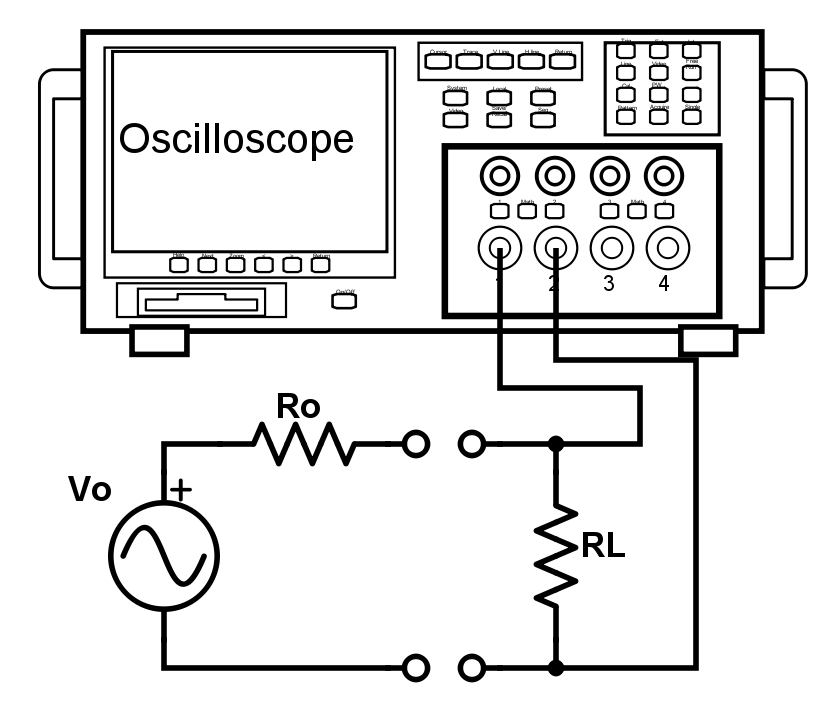
\includegraphics[scale=0.25]{output.png}  
    \caption{This circuit is designed to discover the norton current with can give rise to $R_{o}$ if $V_{o}$ is measured separately.}
\end{figure}

This type of measurement can be made on any circuit. For the second part of the lab, the same set up can be used where $V_{o}$ and $R_{o}$ are the output voltage and output impedance of the circuit created for the second part of the lab.

Op amps are acitve circuit elements that can be used in a multitude of ways. The most important property of an op amp is that the positive and negative terminals of the op amp will be equal. This means that since the positive terminal is grounded, the voltage of the positive and negative terminal will both be zero. This means that $\frac{V_{in}}{R_{in}} = -\frac{V_{out}}{R_{F}}$. Given the definition of the gain we obtain:

\begin{equation}
gain =  \frac{V_{out}}{V_{in}} = -\frac{R_{F}}{R_{in}}
\end{equation}

The invertive amplifier built for this lab is shown below:

\begin{figure}[h]
    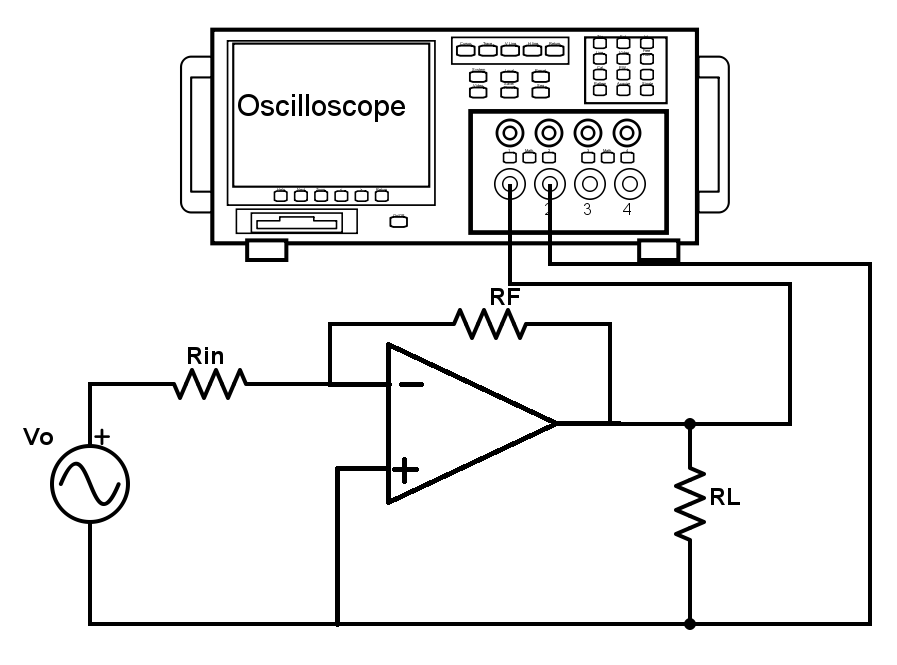
\includegraphics[scale=0.4]{inverting.png}  
    \caption{This circuit is both a high pass filter and an amplifer.}
\end{figure}

For the third part of the lab, a high pass filter and amplifer was made with the op amp. This circuit is shown below. This circuit is a high pass filter because the capacitor only allows high freqency voltages to pass through. In a DC circuit, a capacitor will simply be charged and no current will flow after. In an AC cuircuit, changes in the voltage across the capacitor on one side will cause changes in voltage on the other side. This will allow the AC current to flow through the capacitor. Since the capacitor responds to changes in voltage, higher freqency voltages will pass through the circuit mor easily than low frequency voltages. This is the reason that a circuit in this situation will act as a high pass filter. In this circuit, since there is a negative feedback, the postivie and negative terminals of the op amp will have an equal voiltage. Again, since the positive terminal is grounded, the voltage of the positive and negative terminal will both be zero. Again the gain of this circuit will be determined by:

\begin{equation}
gain =  -\frac{Z_{F}}{Z_{in}}
\end{equation}

This time however, these are complex imedances. In this case, $Z_{in} = R_{in} + C_{in}$. The magnitude of this gain will depend on the frequency of the input voltage. The filter will allow high frequency voltages to pass and low frequencies will have a gain of less than one. The characteristic frequency of an RC circuit is given below:

\begin{equation}
\omega_{RC} =  \frac{1}{R\omega}
\end{equation}

 The op amp circuit built for this part of the lab is shown below:

\begin{figure}[h]
    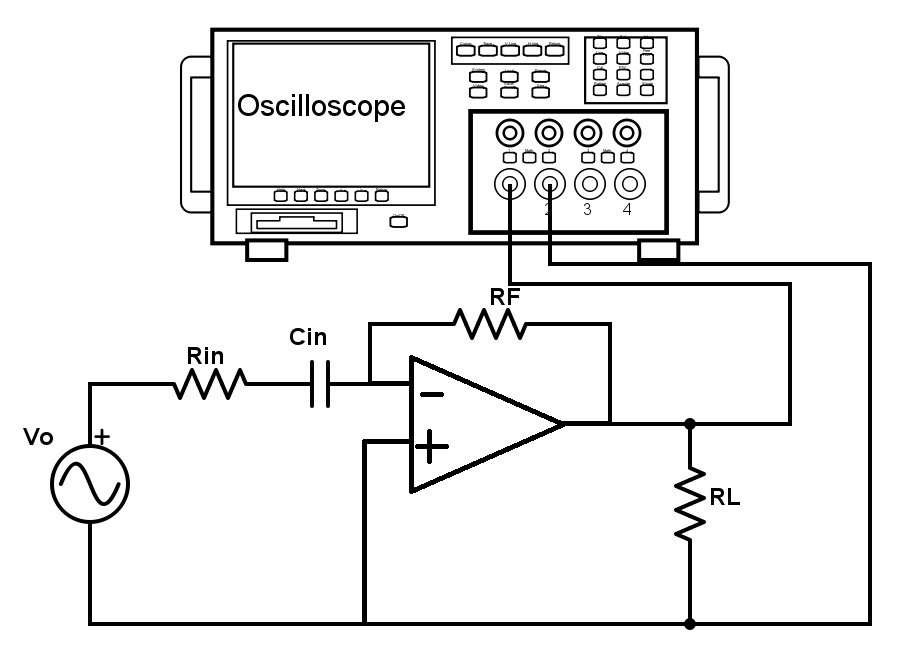
\includegraphics[scale=0.4]{highpassamp.png}  
    \caption{This circuit is both a high pass filter and an amplifer.}
\end{figure}


\section{Methodology}

\begin{enumerate}
    \item Connect the oscilloscope directly to the Protoboard AC voltage supply and mneasure the output voltage.
    \item Set up the circuit shown in figure (1) record the voltage across the resistor and record the resistor value
    \item Build the op amp circuit from figure (2).
    \item Take record of the output voltage with no load attatched.
    \item Add a load to the circuit with a large value as to emilinate sag.
    \item Measure the voltage across the load resistor and the value of this resistor.
    \item Change the frequency and take nots on any changes in the plot on the oscilloscope.
    \item Change the load resistor and investigate the limitations fo the circuit.
    \item Build the circuit from figure (3).
    \item Take recordings of output voltage as the frequency is varied and the input voltage is kept constant.
\end{enumerate}


\section{Results and Analysis}

\subsection{Data}
The half wave rectifier was investigated with various input voltages and frequencies. All voltages for $V_{in}$ and $V_{out}$ were maximum voltages.

The input source was initially set to an amplitude of 2.64V and frequency 7.225Hz. The $V_{out}$ measured across the diode was 1.80V.

\begin{figure}[h]
    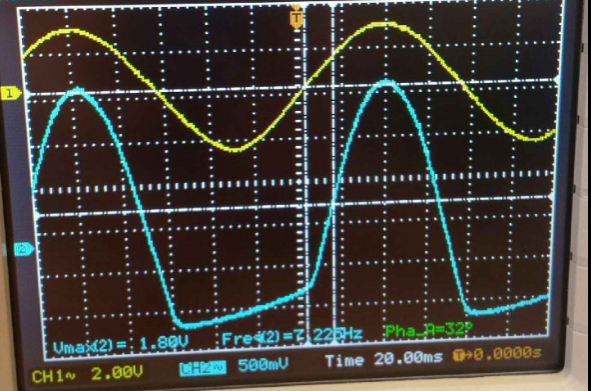
\includegraphics[scale=0.4]{1800mV.png}  
    \caption{$V_{in}= 2.64V$, $f=7.225Hz$, $V_{out} = 1.80V$}
\end{figure}




\section{Conclusion}
The first part of the lab was completed successfully as the group was able to demonstrate that a diode can be used to create close to half of a DC voltage supply. The group discovered that for higher frequency input voltages the plot was more flat on top and bottom. The correct properties of the diode were demonstrated in this part of the lab. When then 3V DC source was added, the results were accurate as the voltage varied between zero and the diode voltage. This is what would have been expected for input voltages below 3V. Results for voltages above 3V were not obtained. This could be done in future labs.

A full wave rectifier was successfully constructed. Its behavior was as expected, creating an all positive voltage output by inverting the negative input voltage. 

The Zener diode portion of the lab was also successful. The Zener voltage behavior was observed by measuring the output voltage while varying the DC input voltage. Then the clipping effect of the Zener diode on half of the waveform was observed by providing a single Zener diode with an AC voltage input. Then, using two diodes in opposite bias directions, the both the positive and negative output voltages were clipped.

Overall, the lab was completed with a large degree of success.



\end{document}

